\chapter{Introduction}

\section{On AI, Computational Linguistics, universe and everything}
%todo:remove, copied in intro 2.0
In 1950 Alan Turing in a seminal paper \citep{Turing1950} published in Mind was asking if ``machines can do what we (as thinking entities) can do?'' He questioned what intelligence was and whether it could be manifested in machine actions indistinguishable from human actions. 

He proposed the famous \textit{Imitation Game} also known as the \textit{Turing test} in which a machine would have to exhibit intelligent behaviour equivalent or indistinguishable from that of a human. The test was set up by stating the following rules. The machine (player A) and a human (player B) are engaged in a written \textit{natural language} conversation with a human judge (player C) who has to decide whether each conversation partner is human or a machine. The goal of players A and B is to convince the judge (player C) that they are human. 

This game underpins the question whether ``a computer, communicating over a teleprinter, (can) fool a person into believing it is human?'', moreover, whether it can exhibit (or even appear to exhibit) human(-like) cognitive capacities \citep{Harnad1992}. Essential parts of such cognitive capacities and intelligent behaviour that the machine needs to exhibit are of course the linguistic competences of comprehension (or ``understanding'') and generation of ``appropriate'' responses (for a given input from the judge C).

The \textit{Artificial Intelligence} (AI) field was born from dwelling on Turing's questions. The term was coined by McCarthy for the first time in 1955 referring to the ``science and engineering of making intelligent machines'' \citep{McCarthy1955}.

The general target is to program machines to do with language what humans do. Various fields of research contribute to this goal. Linguistics, amongst others, contributes with theoretical frameworks systematizing and accounting for language in terms of morphology, phonology, syntax, semantics, discourse or grammar in general. In computer science increasingly more efficient algorithms and machine learning techniques are developed. Computational linguistics provides methods of encoding linguistically motivated tasks in terms of formal data structures and computational goals. In addition, specific algorithms and heuristics operating within reasonable amounts of time with satisfiable levels of accuracy are tailored to accomplish those linguistically motivated tasks.

\textit{Computational Linguistics} (CL) was mentioned in the 1950 in the context of automatic translation \citep{Hutchins1999} of Russian text into English and developing before the field of Artificial Intelligence proper. Only a few years later CL became a sub-domain of AI as an interdisciplinary field dedicated to developing algorithms and computer software for intelligent processing of text (leaving the very hard questions of intelligence and human cognition aside). 
%Besides \textit{machine translation} CL incorporates a broader range of tasks such as \textit{speech synthesis and recognition, text tagging, syntactic and semantic parsing, text generation, document summarisation, information extraction}, etc. 

This thesis contributes to the field of CL and more specifically it is an advancement in \textit{Natural Language Parsing} (NLP), one of the central CL tasks informally defined as the process of transforming a sentence into (rich) machine readable syntactic and semantic structure(s). Developing a program to automatically analyse text in terms of such structures by involving computer science and artificial intelligence techniques is a task that has been pursued for several decades and still continues to be a major challenge today. This is especially so when the target is \textit{broad language coverage} and even more when the desired analysis goes beyond simple syntactic structures and towards richer functional and/or semantic descriptions useful in the latter stages of \textit{Natural Language Understanding} (NLU). 

In computational linguistics, broad coverage natural language components now exist for several levels of linguistic abstraction, ranging from tagging and stemming, through syntactic analyses to semantic specifications. In general, the higher the degree of abstraction, the less accurate the coverage becomes and, the richer the linguistic description, the slower the parsing process is performed. 

Such working components are already widely used to enable humans to explore and exploit large quantities of textual data for purposes that vary from the most theoretical, such as understanding how language works or the relation between form and meaning, to very pragmatic purposes such as developing systems with natural language interfaces, machine translation, document summarising, information extraction and question answering systems to name just a few. 

% end copied 

These software programs originally were designed by and for domain experts but over time the fruits of the technological advancement became available to millions of ordinary people. In a world such as ours, where technology is ubiquitous and pervasive in almost all aspects of our life, natural language processing and understanding becomes of great value and importance regardless whether it materializes as a spell-checker, (not so) clever machine translation, voice controlled car, intelligent assistants such as Siri, Alexa or Google Now . 

\section{The goal of the thesis}
%todo remove
This thesis aims at a reliable modular method for parsing unrestricted English text into a feature rich constituency structure using Systemic Functional Grammars (SFGs).

%aspects to consider
Before describing the parsing method, the following aspects need to be clarified first: the theoretical framework and its descriptive power, the depth and meaningfulness of the analysis, the computational complexity of the process and the level of accuracy and how it is measured. I address each of these aspects in the following chapters and before advancing any further I would like to illustrate through an example of what parsing is. 

\section{An example of Systemic Functional analysis}
%todo copied entirely
\label{sec:example}
This section provides a taste of what does a systemic functional analysis looks like. I provide a parallel analysis between SFL and a traditional grammar in order to highlight the richness and high descriptive potential of SFGs. A source of the descriptive abundance in SFL is achieved through a practice of feature systematisation as mutually exclusive choices which is exemplified for three features of traditional grammar below. The SFL feature analysis provided here is partial and restricted to only two constituents as this suffices to provide the reader with an intuition of what to expect from an SFL analysis. 

Traditional linguistics teaches us how to carry on a syntactic analysis of a sentence. So let's consider Example \ref{ex:1} in order to perform one. First, we focus on clustering words together into constituents guided by the intuitive rule \textit{which word stands goes together with} within the sentence resulting in a grouping such as in Example \ref{ex:2}. 

\begin{exe}
    \ex\label{ex:1} He gave the cake away.
    \ex\label{ex:2} ( (He) (gave) ((the) (cake)) (away) (.) ) 
\end{exe}

%The word ``He'' is closest to ``gave'' and it seems that they go together especially that if we try to group ``He'' and ``the'' they do  sense at all. Then, using sequential proximity criteria, ``gave'' must be related to ``the'' but they do not stick together at all it is rather ``the'' and ``cake'' that are a unity. So ``the'' has a stronger relation to ``cake'' than ``gave''. But actually ``cake'' seems connected to ``gave'' and not the other way around, so the direction of connection seems to matter just as much as its strength. So we see that the sequential proximity sometimes indicated relatedness between words but often it does not. The strength and direction as well are crucial and tt is some sort of meaning making that governs the grouping process. This grouping into syntactic constituents can be expressed using bracketed notation as in Example \ref{ex:2}.


\begin{figure}[!ht]
	\centering
	\begin{tikzpicture}[tree-style,level 1/.style={sibling distance=4em},
	level 2/.style={sibling distance=4em}, level distance=4.5em]
	\node (cla) [pattern-node] {\textit{He gave the cake away.}}
	child { node (sub)[pattern-node] {He}}		
	child { node (mv)[pattern-node] {gave}}
	child { node (com)[pattern-node] {\textit{the cake}}
		child { node (det)[pattern-node]{the}}
		child { node (nou)[pattern-node]{cake}}}
	child {node[pattern-node](adjunct)
		{away}
	};
	\end{tikzpicture}
	\caption{Representation of the Example \ref{ex:2} as constituency tree}
	\label{fig:mcg-graph-example-simple-structure}
\end{figure}

Figure \ref{fig:mcg-graph-example-simple-structure} depicts the constituency division of the clause which is identical to the bracket notation in Example \ref{ex:2}. The nodes represent grammatical constituents and the edges stand for the structure-substructure composition. 

Next we can move on to assign constituent class and a grammatical function. Table \ref{tab:sfg-constituency-analisys} provides a constituency analysis in SFL tradition. Here the sentence is formed of a single clause which has four constituting functional parts: a Subject, a Main Verb (also known as Predicate), a Complement and an Adjunct. Each of these functional parts is filled correspondingly by a pronoun, a verb, a nominal group and an adverb as assigned in the table below.

\begin{table}[!ht]
    \centering
    \begin{tabular}{cc|c|c|c}
        \hline
        \multicolumn{1}{|c|}{\textit{He}} & \textit{gave} & \textit{the}     & \textit{cake}   & \multicolumn{1}{c|}{\textit{away.}} \\ \hline
        \multicolumn{5}{|c|}{clause}                                                                                                 \\ \hline
        \multicolumn{1}{|c|}{Subject}     & Main Verb     & \multicolumn{2}{c|}{Complement}    & \multicolumn{1}{c|}{Adjunct}        \\ \hline
        \multicolumn{1}{|c|}{pronoun}      & verb          & \multicolumn{2}{c|}{nominal group} & \multicolumn{1}{c|}{adverb}         \\ \hline
        &               & Deictic          & Thing           &                                     \\ \cline{3-4}
        &               & determiner       & noun            &                                     \\ \cline{3-4}
    \end{tabular}
    \caption{Constituency analysis with unit classes and grammatical functions}
    \label{tab:sfg-constituency-analisys}
\end{table}

Next each constituent can be assigned a set of relevant features. For example The subject ``He'' is a pronoun that has features known in traditional grammar: \textit{singular}, \textit{masculine}, and \textit{3^{rd} person}. These features are well differentiated in traditional grammar. For example \textit{singular} means \textit{non-plural}, \textit{masculine} means \textit{non-feminine} and \textit{3^{rd} person} means \textit{non-1^{st}} and \textit{non-2^{nd}}. These are closed classes meaning that there is no \textit{4^{th} person} or that there is no \textit{neutral} grammatical gender in English as other languages have. These features can be systematised (see Figure \ref{fig:traditional-pronoun}) as three systems of mutually exclusive choices that can be assigned to pronominal units. Note that the gender is enabled for 3^{rd} person singular pronouns which can be expressed as is the figure below representing a \textit{system network} (which is properly introduced in Chapter \ref{ch:sfg}).

\begin{figure}[!ht]
    \centering      
    \includegraphics[width=.56\textwidth]{Figures/Example/traditional-pronoun.pdf}      
    \caption{The systematisation of three pronominal features in traditional grammar}
    \label{fig:traditional-pronoun}
\end{figure}

In SFG the pronouns are systematised in the system network of Person from \textit{Introduction to Functional Grammar} \citep[366]{Halliday2013} that is depicted in Figure \ref{fig:person-system-network}. The red rectangles from the figure represent the selections that are applicable to the Subject constituent ``He'' in example above.

\begin{figure}[!ht]
    \centering      
    \includegraphics[width=.90\textwidth]{Figures/Example/person-selections.pdf}      
    \caption{The selections in Person system network from \citet[366]{Halliday2013} }
    \label{fig:person-system-network}
\end{figure}

Lets take now the clause constituent that is the root of the constituency tree and see how SFL features can be applied to it. If in in terms of traditional grammar the clause can be ascribed relatively few features i.e. as having \textit{passive voice}, \textit{positive polarity} and \textit{simple past tense} then in terms of SFL grammar the features are many more i.e. \textit{major, positive, active, effective, receptive, agentive, free, finite, temporal, past, non-progressive, non-perfect, declarative, indicative, mood-non-assessed, comment-non-assessed}. Figure \ref{fig:mood-selections} depicts the selections applicable to clause constituent in Example \ref{ex:1} from Mood system network that is an adaptation of Mood network proposed in \citet[162]{Halliday2013}. 

\begin{figure}[!ht]
    \centering      
    \includegraphics[width=0.91\textwidth]{Figures/Example/mood-selections.pdf}      
    \caption{The systematisation of three pronominal features in traditional grammar}
    \label{fig:mood-selections}
\end{figure}

So far you have seen constituents assigned syntactic functions such as Subject, Complement, Adjunct etc. SFL covers a wider range of functions depending on the kind of meaning it aims at describing. For example what in other grammars is known as \textit{semantic labels}, \textit{thematic} or \textit{$\theta$ roles} SFL systematises as Transitivity system network (which will be introduced in Chapter \ref{sfg} below). Transitivity aims at providing domain independent \textit{semantic frames} called in SFL \textit{process configurations} which describe semantic actions and relationships, along with \textit{semantic roles} ascribed to their \textit{participants}. These semantic frames generally are governed by verbs and more specifically each verb meaning has a dedicated semantic frame. 

For example \ref{ex:1} corresponds to a Possessive semantic frame where ``He'' is the Agent and Carrier whereas ``the cake'' is the Possessed thing as marked in Example \ref{ex:3}. These configurations and participant roles correspond to Transitivity system network proposed in \citep{Neale2002}.

\begin{exe}
    \ex\label{ex:3} [_{Agent-Carrier} He] gave [_{Possessed} the cake] away. 
\end{exe}

There are more functions and features that can be assigned to the constituents in the Example \ref{ex:1} but I stop here. The analysis provided so far highlights that SFG grammar has a variety of functions serving to express different meanings. The traditional grammar distinguishes them as syntactic and semantic functions but, as we will see in Chapter \ref{ch:sfg} below, SFL does not make such a distinction. Another aim of the current section was to provide a glance of the feature rich grammar and I hope the example with Mood feature selection in Figure \ref{fig:mood-selections} fulfils this goal.

\begin{figure}[!ht]
	\centering
	\begin{tikzpicture}[scale=0.8, transform shape, tree-style, 
		level 1/.style={sibling distance=11em, level distance=14em},
		level 2/.style={sibling distance=10em, level distance=12em}, 
		anchor=north
		growth parent anchor = north,]

	\node (cla) [pattern-node, split-node, text width = 42em,]  
		{clause 
		\nodepart{two} Configuration
		\nodepart{three} major, positive, active, effective, receptive, agentive, free, finite, temporal, past, non-progressive, non-perfect, declarative, indicative, mood-non-assessed, comment-non-assessed, posessive};

		\node (sub) [pattern-node, split-node, below=3em of cla, xshift=-16em,] 
			{pronoun
			\nodepart{two} Subject, Participant,\\ 
                            Agent \& Carrier 
			\nodepart{three} 3^{rd} person, singular,\\ 
                             male, non-interactant,\\ 
                             one-referent, conscious};

		\node (mv)[pattern-node, split-node, below=3em of cla, xshift=-5em] 
			{verb
			\nodepart{two} Main Verb, Finite, \\Process 
			\nodepart{three} possessive };

		\node (com)[pattern-node,split-node, below=3em of cla, xshift=6em] 
			{nominal group
			\nodepart{two} Complement, Participant, 
                            \\ Affected \& Possessed
			\nodepart{three} };

		\node (det)[pattern-node,split-node, below=3em of com, xshift=-6em]
			{determiner
				\nodepart{two} Deictic, Modifier
				\nodepart{three} specific, demonstrative,\\ 
                                 determinative, non-selective};

		\node (nou)[pattern-node,split-node, below=3em of com, xshift=6em]
			{noun
				\nodepart{two} Thing, Head
				\nodepart{three} inanimate, singular,\\ 
                                 countable };

		\node[pattern-node,split-node, below=3em of cla, xshift=17em](adjunct)
			{adverb
			\nodepart{two} Adjunct,
                           \\Circumstance,
                           \\Location
			\nodepart{three} };

		\draw[sequence,-,edge-style] (cla.south) -- ++(0,-1em) -| (sub.north);
		\draw[sequence,-,edge-style] (cla.south) -- ++(0,-1em) -| (mv.north);
		\draw[sequence,-,edge-style] (cla.south) -- ++(0,-1em) -| (com.north);
		\draw[sequence,-,edge-style] (cla.south) -- ++(0,-1em) -| (adjunct.north);
		\draw[sequence,-,edge-style] (com.south) -- ++(0,-1em) -| (det.north);
		\draw[sequence,-,edge-style] (com.south) -- ++(0,-1em) -| (nou.north);	
	\end{tikzpicture}
	\caption{Representation of Example \ref{ex:1} as feature rich constituency graph}
	\label{fig:mcg-graph-example}
\end{figure}


Next, Figure \ref{fig:mcg-graph-example} summarises everything discussed above into a partially filled constituency tree. The constituents that were not discussed are assigned only few high level features.
%Each constituent can be decorated with its grammatical features . For example the word ``he'', we know, is third person pronoun, masculine gender and singular number; or the word ``gave'' is a verb and the predicate of the sentence, and so on. 
%The structure in Figure \ref{fig:mcg-graph-example} depicts a syntactic constituency tree in which 
In Figure \ref{fig:mcg-graph-example} every node is richly decorated with syntactic and semantic features. The blue part of each node denotes grammatical class, the red part carries functions some of  which are important to establishing a valid constituency structure (that are Mood functions) and the the Transitivity functions; and the green part some grammatical features selected from system networks. In practice, the feature set is much richer than what nodes in Figure \ref{fig:mcg-graph-example} carry here the restriction aims simply to avoid an over-crowded example. Generating automatically feature rich constituency structure such as the one in Figure \ref{fig:mcg-graph-example} is the general purpose of the current work.

Next ...

\section{The linguistic framework}
%todo copied already to 2.0
% the linguistic framework
%% on SFL
Any description or analysis involving language implies some theory of how language works. In this thesis I chose the Systemic Functional Linguistic (SFL) framework because of its versatility in producing descriptions along \textit{multiple semiotic dimensions} \citep{Halliday2003} (i.e. paradigmatic, syntagmatic, meta-functional, stratification and instantiation dimensions) and at different \textit{delicacy levels} of the \textit{lexico-grammatical cline} \citep{Halliday2002, Hasan2014}. 

%I discuss theoretical and pragmatic aspects of Systemic Functional Grammar (SFG) and explain it more detail in Chapter \ref{ref}.

% deeper on SFL
SFL regards language as a social semiotic system where any act of communication is regarded as a conflation of \textit{linguistic choices} available in a particular language. Choices are organised on a paradigmatic rather than structural axis and represented as \textit{system networks}. Moreover, in the SFL perspective language has evolved to serve particular \textit{functions} influencing their the structure and organisation of the language. However, their organisation around the paradigmatic dimension leads to a significantly different functional organisation than those found in several other frameworks which \citet{Butler2003-pt1, Butler2003-pt2} treats extensively. 

Elaborating the foundations laid by his British teacher J. R. Firth, \citet{Hjelmslev53} from Copehagen School of linguistics and a group of European linguists from Prague School, Halliday develops the beginnings of SFL in his seminal paper \cite{Halliday61-orig}. Inspired by \textit{oragnon model} formulated by \citet{Buhler34}, Halliday refers to the language functions as metafunctions or lines of meaning offering a trinocular perspective on language through \textit{ideational}, \textit{interpersonal} and \textit{textual} metafunctions.
%such as Prague School, Lexical Functional Grammar, Head-driven Phrase Structure Grammar (HPSG), Role and Reference Grammar, Functional Discourse Grammar and others
In SFL, language is first of all an interactive action serving to enact social relations under the umbrella of the \textit{interpersonal metafunction}. Then it is a medium to express the embodied human experience of inner (mental) and outer (perceived material) worlds via \textit{ideational metafunction}. Finally the two weave together into a coherent discourse flow whose mechanisms are characterised through the \textit{textual metafunction}.

% on metafunctions
%TODO briefly introduce and refere to other extensive sources
%To account for the complexity and phenomenological diversity of human language the SFL theory provides descriptions along \textit{syntagmatic, (meta)functional, paradigmatic, stratification and instantiation axes}. 

% 
There are two models of SFG: the \textit{Sydney Grammar} developed by \citet{Halliday2013}, the founding fathers of \textit{Systemic Functional Linguistics} (SFL), and \textit{Cardiff Grammar} developed by \citet{Fawcett2008}, an extension and in a way simplification of Sydney Grammar. Each of the two grammars has advantages and shortcomings which I present in analyse and select based on theoretical soundness and suitability to the goals of the current project.

Cardiff and Sydney grammars had been used as language models in natural language generation projects within 
the broader contexts of social interaction. Some researchers \citep{Kasper1988, ODonoghue1991a, ODonnell1993, Souter1996, Day2007} attempted to reuse the grammars for the purpose of syntactic parsing within the borders of NL generation coverage. I come back to these works in more detail in Section \ref{sec:sota}.

\section{The SFG complexity problem}
%todo copied
Given the thorough explanations of \citet{Bateman2008} of the reasons for such tremendous complexity after the attempts of \citet{Kasper1988}, \citet{Kay1985}, \citet{ODonoghue1991a}, \citet{ODonnell1993} and \citet{Day2007}, to mentiona few, none of which managed to parse broad coverage English with full SFG and without aid of some sort. Each had to accept limitations either in grammar or language size and eventually using simpler syntactic trees as a starting point of the parsing process. So what is it about? 

Automatic analysis of text can be seen as a problem of searching though the space of possible solutions for an appropriate or even optimal solution. Here we speak of the Systemic Functional Grammar as a linguistic resource that shapes the search space and the way it access to that space is available. The systemic lexicogrammar is organised paradigmatically and was proven to be a good structure for natural language generation task but it turns out to be unusable for the reverse problem, that of natural language analysis. The principal issues is that of handling the \textit{search space} leading back to Halliday's question ``How big is a grammar?'' \citep{Halliday66-deep}.

The size of the search space defined by a grammar depends on the number of system networks and on the kind of connectivity and cross-classification it provides. For example given 50 system networks, the size of the search space lies somewhere between 51 and 2^{50}. This nevertheless is not such a big deal in the case of generation, as \citet{Halliday96-grammatics} says that the ``number of choice points [...] is actually rather small'' as only few of the actual possibilities produced by a system network need to be explored when generating a clause. ``Possible feature selections become relevant only when they are revealed to be relevant by prior paradigmatic choices and it is only those alternatives that need to be considered''\citep{Bateman2008}.

Analysis is not symmetric with generation and the paradigmatic context of choice that is available during generation is no longer accessible in parsing. It is not known any longer which features of a systemic network are relevant and which are not. That is: in generation, the simple traversal of the network finds only the compatible choices because that is what the network leads to; whereas in analysis it is not evident in advance which path to follow therefore the task is virtually to explore entire search space in order to discover which features apply to the text \citep{Bateman2008}.

%\section{Towards broader solution: reduce search space and guide systemic traversal in parsing}
%todo copied

In the analysis task first difficulty that needs to be addressed is discovering from a sequence of words what possible groups are combinable into grammatical groups, phrases or clauses. This is a task of bridging a sequence of words input and the grammatical description of \textit{instantial syntagmatic organizations} involving \textit{configurations of grammatical functions}. In a second stage these grammatical functions can serve as paradigmatic context for further traversing the system network and extend to the full set of systemic features. Moreover they will play a crucial role in restricting and organising the search space for relevant and applicable network parts during analysis task.

Addressing the gap of the syntagmatic account within the SFG framework, can be done by, first, providing information about which grammatical functions operate at each rank, second which grammatical functions can be filled by which classes of units and third by providing relative and absolute account of ordering within each unit structure. This sort of information can guide the building of a constituency backbone structure. As a second stage, as mentioned above, the unit classes and grammatical functions can operate as ``hooks'' on system network to guide the traversal in the same way the paradigmatic context available in the generation process. 

Alternatively the problem of structure construction can be outsourced for parsing with other grammars. Then the problem changes into creating a transformation mechanism to obtain the SFL constituency structure rather than build it from scratch. Starting the SFG parsing process from a syntactic tree produced with other grammars reduces the computational complexity of the task and reduce the search space. 

The second stage of constituent enrichment by network traversal can be further aided by checking an arbitrary set of patterns for preselecting even more features recoverable via lexico-syntactic patterns.
%This approach is integrated 
%and shifts the focus to recognising grammatical features in the patterns of syntactic structures, morphological forms and lexical choices. 
%pattern recognition flash out: comparative of SFG features to simpler grammars where those are implicit
%The grammatical variations are paradigmatically systematized in SFG. Generative or dependency grammars account for variations in syntactic structure. The latter can them rather implicitly through structure and not explicitly through features. 
%Those variations can be identified as lexico-syntactic patterns (lexical and syntagmatic) which stand for a set of feature selections rather than a single one. 
The pattern recognition plays an essential role in current parsing method for fleshing out the constituent backbone with systemic selections.

\section{The Opportunity}
\label{sec:opportunity}
\todo[inline]{
    Second, a large amount of description of this kind has
    traditionally been done, and done a lot, in SFL. Here again
    you need to find a good collection of example 'applications'
    in SFL (not computational) where the deeper analysis
    has been found useful and give references: education,
    text/discourse analysis (critical)\citep{Tenorio2011} [Encarnacion Hidalgo Tenorio 2011, Critical Discourse Analysis, An overview], whatever plus references.
    
    Survey of studies in systemic functional language description \citep{Mwinlaaru2016}
    
    functional information is found useful for text analysis, but this has only been done informally
    
    well, look at the education work, the typology work,
    the CDA work: these are the main areas where SFL appears
    and has papers.
}
%TODO: add material from Martin2000-close, Martin2000-practice, Bateman2017-sfl

Critical Discourse Analysis from it's inception was designed, but is not limited to, questioning the status quo by detecting, analysing and also resisting enactments of power abuse as transmitted in private and public discourses. The philosophical and linguistic bases on which CDA is grounded are certain branches of social theory and earlier discourse analysis, text linguistics and interactional sociolinguistics. CDA seeks to expose the manipulative nature of discursive practices, and improve communication and well-being by removing the barriers of assumed beliefs legitimised through discourse\citep{Tenorio2011}. 

SFL theory of language has been widely adopted in CDA community. It comes handy when one and the same piece of reality is portrayed differently depending on the side and role of the source. For example one and the same historical event can be described as a riot, demonstration, or a protest. For the same reason various agents can be either presented as antagonists that instigate the conflict or protagonists that oppose it by simple selections of grammatical coding. Thus different linguistic descriptions lead to different constructions of the reality. 
%Controlling and knowing how to manipulate these constructions leads to accumulation and hold of power. 


\section{On theoretical compatibility and reuse}
\label{sec:reuse}
%todo copied 
% reuse motivation, context to parsing 
In the past decades many significant progresses have been made in natural language parsing framed in one or another linguistic theory each adopting a distinct perspective and set of assumptions about language. The theoretical layout and the available resources influence directly what is implemented into the parser and each implementation approach encounters challenges that may or may not be common to other approaches in the same or other theories. 

Parsers implementing one theoretical framework may face common or different problems to those implementing other theories. The same can be said of the solutions. When a solution is achieved using one theory it is potentially reusable in others. The successes and achievements in any school of thought can be regarded as valuable cross theoretical results to the degree links and correspondences can be established. Therefore reusing components that have been shown to work and yield ``good enough results'' is a strong pragmatic motivation in the present work.

%
This thesis employs three linguistic frameworks namely the \textit{Systemic Functional Linguistics}, \textit{Dependency Grammar} and \textit{Governance \& Binding Theory}. SFL has already been motivated in Section \ref{sec:framework} and is introduced in detail in Chapter \ref{ch:sfl}. The other two frameworks are employed because some of the accomplishments using them are directly reused in this thesis and I explain below how. Chapter \ref{ch:dependecy-grappamr} and \ref{ch:gbt} besides introducing the Dependency grammar and correspondingly Government and Binding Theory show how these frameworks relate to each other and to which degree they are compatible to undergo a conversion process for the purpose of reuse.

%The compatibility
%It demonstrates how selected grammatical frameworks namely \textit{Systemic Functional Grammar}, \textit{Dependency Grammar} and \textit{Governance \& Binding Theory} relate to each other and to which degree they are compatible to undergo a conversion process and to show that simple patterns carrying grammatical information can be used to enrich syntactically and semantically the parse structures. And here is a brief motivation for selecting these frameworks.   

%
In the last years \textit{Dependency Grammar} \citep{Tesniere2015} became quite popular in natural language processing world favoured in many projects and systems. The grammatical lightness and the  modern algorithms implemented into dependency parsers such as Stanford Dependency Parser \citep{Marneffe2006}, MaltParser \citep{Nivre2006}, MSTParser \citep{McDonald2006} and Enju \citep{Miyao2005} are increasingly efficient and highly accurate. Among the variety of dependency parsing algorithms, a special contribution bring the \textit{machine learning} methods such as those described in \citet{mcdonald2005online, mcdonald2006online, carreras2007experiments, zhang2011transition, pei2015effective} to name just a few. 

As the dependency parse structures provide information about functional dependencies between words and grants direct access to the predicate-argument relations and can be used off the shelf for real world applications. 
This information alone, would makes the dependency grammar a suitable candidate to supplement the syntagmatic account missing in SFGs and provide some functional hooks for reducing complexity in parsing with SFGs. Hence once of the goals in this work is investigating to which degree the dependency grammar is structurally and functionally compatible with SFGs to undergo a cross theoretic transformation. This hypothesis is theoretically investigated in Chapter \ref{ch:dependecy-grammar} and then evaluate empirically in Chapter \ref{ch:evaluation}. The investigation is based specifically on Stanford Dependencies parser version 3.5 \citep{Marneffe2008a,Marneffe2008, Marneffe2014}. 

%todo end of copied 

Regardless of being a simple grammatical framework which accounts for the syntactic relations between words, the Stanford dependency grammar is structurally and functionally compatible to SFG. 
The account it provides for the word dependencies can be viewed also in functional terms and I expand this idea in Chapter \ref{ch:dependecy-grappamr}. It is a much more suitable foundation for building the SFG syntactic structure than phrase-structure trees, as well as for making more delicate grammatical distinctions (a process highlighted in Section \ref{sec:how-works} and explained in detail in Chapter \ref{ch:parsing-algorithm}).

The current parsing process requires accounting for \textit{null elements} which are not covered by the dependency  grammar. As a solution I turned to a part of Chomsky's Transformational Grammar\citep{Chomsky1957}, Government and Binding Theory (GBT) \citep{Chomsky81,Haegeman1991}, to identify and create the Null Elements to support the semantic parsing. I introduce GBT and provide inter-grammatical links between towards dependency grammar in Chapter \ref{ch:gbt}.

Current work is the first one to parsing with a dependency backbone, all previous ones using context-free grammars. 
There are other good candidates to serve as backbone (CCG, TAG, FCG, HPSG etc.) but a broad investigation of parsers and the compatibility of their linguistic theoretical frameworks to SFL is outside the scope of this thesis. 

\section{Previous works on parsing with Systemic Functional Grammars}
%todo:remove: copied to cahpter file
\label{sec:sota-old}
There have been various attempts to parsing with SFGs. This section covers the most significant attempts to parse with a Systemic Functional Grammar. The firs attempt was made by Winograd \citep{Winograd1972} which was more than a parser, it was an interactive a natural language understanding system for manipulating geometric objects in a virtual world.

Starting from early 1980s onwards, Kay, Kasper, O'Donell and Bateman tried to parse with Nigel Grammar \citep{Matthiessen1985}, a large and complex natural language generation (NLG) grammar for English used in Penman generation project. Other attempts by \citet{ODonoghue1991a}, \citet{Weerasinghe1994}, \citet{Souter1996}, \citet{Day2007} aim for corpus based probability driven parsing within the framework of COMMUNAL project starting from late 1980s.

In a very different style, \citet{Honnibal2004a,Honnibal2007} constructed a system to convert Penn Treebank into a corresponding SFGBank. This managed to provide a good conversion from phrase structure trees into systemic functional representation covering sentence mood and Thematic constituency (a kind of analysis in SFL which is not considered in current work). Transitivity has not been covered there because of its inherently semantic nature but it is in the current work.

\subsection{Winograd's SHRDLU}
SHRDLU is an interactive program for understanding (if limited) natural language written by Terry Winograd at MIT between 1968-1970. It carried a simple dialogue about a world of geometric objects in a virtual world. The human could as the system to manipulate objects of different colours and shapes and the ask questions about what has been done or the new state of the world. 

It is recognised as a landmark in natural language understanding demonstrating that a connection with artificial intelligence is possible if not solved. However, his success was not due to the use of SFG syntax but rather due to small sizes of every system component to achieve a fully functional dialogue system. Not only it was parsing the input but it was developing an interpretation of it, reason about it and generate appropriate natural language response. 

Winograd combined the parsing and interpretation processes such that the semantic interpreter was actually guiding the parsing process. The knowledge of syntax was encoded in the procedures of interpretation program. He also implemented an ingenious backtracking mechanism where the the program does not simply go back, like other parsers, to try the next possible combination choice but actually takes a decision on what shall be tried next.  

Having data embedded into the program procedures, as Winograd did, makes it non-scalable for example in accommodation of larger grammars and knowledge bodies and unmaintainable on the long term as it becomes increasingly difficult to make changes \citep{Weerasinghe1994}.

\subsection{Kasper}
Bob Kasper in 1985 being involved in Penman generation project embarked on the mission of testing if the Nigel grammar, then the largest available generation grammar, was suitable for natural language parsing. Being familiar with Functional Unification Grammar (FUG), a formalism developed by Kay and tested in parsing \citep{Kay1985} which caught on popularity in computational linguistics regardless of Kay's dissatisfaction with results, Kasper decided to re-represent Nigel grammar into FUG. 

Faced with tremendous computational complexity, \citet{Kasper1988} decided to manually create the phrase-structure of the sentences with hand-written rules which were mapped onto a parallel systemic tree structure. Kasper in \citeyear{Kasper1988} was the first one to parse with a context-free backbone. He first parsed each sentence with a Phrase Structure Grammar (PSG), typical to Chomsky's Generative Transformational Linguistics \citet{Chomsky1957}. He created a set of rules for mapping the phrase structure (PS) into a parallel systemic tree like the one depicted in Figure \ref{fig:kasper-example}. When all possible systemic tree were created they were further enriched using information from Nigel Grammar \citep{Matthiessen1985}.

\begin{figure}
	\begin{tikzpicture}[scale=0.9, transform shape]
	%
	\Tree [.\node (ng) {NG}; 
	[.\node (ngps) {NGPS} ;
	[.\node (ngps1) {NGPS}; 
	[.\node (ngpre) {NGPRE} ;
	[.\node (dn) {DN} ; ]
	[.\node (classif) {CLASSIF} ;]
	]
	[.\node (nghead) {NGHEAD} ;]
	]
	[.\node (pp) {PP}; ]
	]
	]
	
	\node [right=1em of pp, single arrow, draw, black, text width=1em] (arrow) {   };
	
	\node[xshift=17em, yshift=-3em, align=center] (n) {nominal-group-simplex};
	\node[below=3em of n, align=center, xshift=-7em] (d) {DEICTIC \\ deictic};
	\node[below=3em of n, align=center, xshift=-2em] (c) {CLASSF \\ noun};
	\node[below=3em of n, align=center, xshift=2em] (t) {THING \\ };
	\node[below=3em of n, align=center, xshift=9em] (q) {QUALIFIER \\ accompanying-process};
	
	
	\draw[sequence,-] (n.south) -- ++(0,-2em) -| (d.north);
	\draw[sequence,-] (n.south) -- ++(0,-2em) -| (c.north);
	\draw[sequence,-] (n.south) -- ++(0,-2em) -| (q.north);
	\draw[sequence,-] (n.south) -- ++(0,-2em) -| (t.north);
	
	\end{tikzpicture}
	\caption{Transformation from phrase structure into systemic constituency structure. Rule example from \cite{ODonnell2005}.}
	\label{fig:kasper-example}
\end{figure}

Once the context-free phrase-structure was created using bottom-up chart parser it was further enriched from the FUG representation of Nigel grammar. This approach to parsing is called \textit{parsing with a context-free backbone} as phrase-structure is conveyed as simplistic skeletal analysis, fleshed out by the detail rich systemic functional grammar. 

Even though Kasper's system is represents the first attempt to parse with full Hallidayan grammar, it's importance is lowered, as \citet{ODonnell2005} point out, by the reliance on phrase structure grammar.

\subsection{O'Donnell}
Since 1990, Mick  O'Donnell experimented with several parsers for small Systemic grammars,  but found difficulty when scaling up to larger grammars. While working in EAD project, funded by Fujitsu, he recompiled a subset of Nigel grammar into two resources: the set of possible function bundles allowed by the grammar (along with the bundles  preselections) and a resource detailing which functions can follow a particular function \citep{ODonnell1993,ODonnell1994}.

This parser was operating without a syntactic backbone directly from a reasonable scale SFG. However when scaled to the whole Nigel grammar the system became very slow because of the sheer size of the grammar and its inherent complexity introduced by multiple parallel classifications and functional combinations - a problem well described by \citet{Bateman2008}. Then O'Donnell wrote his own grammar of Mood that was more suitable for the parsing process and less complex than the recompiled Nigel.

In 2001, while working in a Belgian company O'Donnell came to conclusion that dependency grammars are very efficient for parsing. Together with two colleagues, he developed a simplified systemic grammar where elements were connected through a single function hence avoiding (functional) conflation. Also the ordering of elements was specified relative to the head rather than relative to each other.

More recently, O'Donnell in UAM Corpus Tool embedded a systemic chart parser \citep{ODonnell2005a} with a reduced systemic formalism. He classifies his parser as a left to right and bottom up with a custom lexicon where verbs are attributed features similar to Hallidayan process types and nouns a unique semantic category like thing-noun, event-noun, location-noun etc.

Because of previously reported complexity problems \citep{ODonnell1993} with systemic grammars, the grammatical formalism is reduced to a singular functional layer of Mood-based syntactic structure (Subject, Predicate, Object etc.) ignoring the Transitivity (Actor/Goal, Sensor/Phenomenon etc.) and  Textual (Theme/Rheme) analyses. %Unificationally, 
O'Donnell deals away with the conflation except for the verbal group system network. He also employs a slot based ordering where elements do not relate to each other but rather to the group head only simplifying the number of rules and calculation complexity.   

In his paper \citep{ODonnell2005a} does not provide a parser evaluation so its accuracy is still unknown today. The lexicon that was created is claimed to deal with word semantic classes but it is strongly syntactically based assigning a single sense to nouns and verbs ignoring the peculiar aspect of language polysemy. Moreover it is not very clear the framework within which the semantic classes have been generated. 

\subsection{O'Donoghue}
O'Donoghue proposes a corpus based approach to parsing using \textit{Vertical Strips} \citep{ODonoghue1991a}. They are defined as a vertical path of nodes in a parse tree starting from the root down to the lexical items but not including those. He extracted the set of vertical strips from a corpus called Prototype Grammar Corpus together with their frequencies and probability of occurrence.
This approach differ from the traditional one with respect to the kind of generalization it is concerned and specifically, the traditional approached are oriented towards horizontal order while the vertical strip approach is concerned with vertical order in the parse tree. 

To solve the order problem O'Donoghue uses a set of probabilistic collocation rules extracted from the same corpus indicating which strips can follow a particular strip. He also created a lexical resource indicating for each word which elements can expanded it.

The parsing procedure is a simple lookup of words in the lexical resource selecting all possible elements it can expound and then selecting possible strips starting with the elements expounded by the word. Advancing from left to right for each sentence word more strips compatible with the previously selected ones are selected within the collocation network constrains. The parser finds all possible combinations of strips composing parse trees representing possible output parses. 

The corpus from which the vertical strips were extracted is 100,000 sentences large and was generated with Fawcett's natural language generation system and was tested on the same corpus leaving unclear how would the parser behave on a real corpus. In 98\% of cases the parser returns a set of trees (between 0 and 56) that included the correct one with an average of 6.6 trees per parse. 

Actually, using a larger corpus could potentially lead to a combinatorial explosion in the step that looks for vertical strips. It would decrease the accuracy of the parse because of the higher number of possible trees per parse.

\subsection{Honnibal}
Honnibal \citeyearpar{Honnibal2004a,Honnibal2007} describes how Penn Treebank can be converted into a SFG Treebank. Before assigning to parse tree nodes synthetic features such as mood, tense, voice and negation he first transforms the parse trees into a form that facilitates the feature extraction. 

The scope of SFG corpus was limited to a few Mood and Textual systems leaving aside Transitivity because of its inherently lexico-semantic nature. He briefly describes how he structurally deals with verb groups, complexes and ellipses as functional structures are much flatter than those exhibited in the original Treebank. Then he describes how are identified metafunctional features of unit class, mood function, clause status, mood type, polarity, tense, voice and textual functions.

The drawback of his approach is that the Python script performing the transformation does not derive any grammar but rather implements directly these transformations as functions falling into the same class of problems like Winograd's SHRDLU. By doing so the program is non-scalable for example in accommodation of larger grammars and knowledge bodies and unmaintainable on the long term as it becomes increasingly difficult to make changes. 


\section{Current approach to parsing}
%todo, needs attention
The main problem in using SFGs for parsing is that they are very large and complex. Some parsing approaches use a syntactic backbone which is then flashed out with SFG description. Other ones use a reduced set or a single layer of SFG representation the third ones use an annotated corpus as the source of a probabilistic grammar. Regardless of the approach each limits the SFG in a one way or another balancing the depth of description with language coverage: that is either \textit{deep description but a restricted language} or \textit{shallow description but broad language coverage}. 

Current approach is aligned with works of Honnibal, Kasper and O'Donnell with respect to using a backbone structure and enriching it with syntactic and semantic features. It relies on parse structures produces in other grammars and then translated to systemic functional constituency structure. The contributions on theoretical compatibility and inter-grammatical transformations are briefed in the Section \ref{sec:reuse} coming up next. 

Current method employs rules for graph traversal in order to build a parallel backbone constituency tree and rules for graph matching to enrich it with systemic features. This aims at keeping the language coverage broad at the expense of higher systemic delicacy. I cover basic Mood systems which is way less than what is available in Nigel grammar and leave it for the future work to extend the grammatical delicacy.

%lexico-semantic features
Nonetheless I attempt to cover some the lexico-semantic features as well. Parsing Transitivity system, a task similar to Semantic Role Labelling, requires large lexicogrammatical resource describing verb meanings in terms of their process type and participant roles. The semantically-oriented decomposition of clauses offered by SFL is still sufficiently closely tied to observable grammatical distinctions as to offer a powerful bridge to automatic analysis. Such descriptions are analogous to frame representations \citep{Fillmore1985} as found in FrameNet \citep{Baker1998} or VerbNet \citep{Kipper2008} applied in Semantic Role Labelling Task \citep{Carreras2005}.

O'Donnell approaches this task by providing possible process types directly to the verb by employing self constructed lexicon where each word has syntactic and semantic features. Only recently a resource comparable to FrameNet and VerbNet has been produced in the SFL framework called Process Type Database (PTDB) \citep{Neale2002}. PTDB which provides for each verb a process configuration (similar to a semantic frames) in terms of process type and participant roles. Current work represents the first attempt of using the PTDB to produce semantic (or Transitivity) analysis which combined with pattern patching method has an advantage over O'Donnell's parser. It enables to simultaneously assign, if matched, the systemic features to all clause constituents or not at all.

Another major advantage, as compared to Honnibal's approach is that the grammar and the program are carefully disconnected so that the code is maintainable and scalable with the respect to size of the grammar. This makes it possible to choose rather pragmatically which graph patterns to consider for parsing depending on the scope of task at hand.

%\section{The parsing depth and meaningfulness}
%%the syntax and semantics
%Transformational-Generative Grammars \citep{Haegeman1991,Radford1997} treat the syntax and the semantics as distinct structures, the latter being a realization of the former via a set of transformations. SFG due to its paradigmatic orientation is a ``semantically significant grammar'' systematizing the meaning potential of a language into a network of choices. The organization as a network of systemic choices spans from the from the most obvious grammatical distinctions down to the most delicate ones which, increasingly, are of deeper semantic nature, arriving at the lexicon as the most delicate level. In fact, \citet{Hasan1996,Hasan2014} presents the idealisation of lexicon as the most delicate grammar.
%
%% a common practive in CL
%It is a common practice in the mainstream natural language processing to instantiate some form of a pipeline process starting with surface structure analysis and then incrementally moving towards deeper and more meaningful analysis. As an approximation, the Natural Language Understanding can be divided into three steps: \textit{syntactic parsing}, \textit{semantic interpretation} and then \textit{conceptual processing in the higher levels of belief and reasoning}. 
%
%In current work I adopt similar pipeline approach. Some parts of the SFG that are closer to surface realizations i.e. to syntactic analysis, in traditional terms, are processed earlier in the pipeline, and the other parts that are closer to what is called semantic (or even pragmatic analysis), run in the latter stages of the pipeline.

%This work addresses both syntactic and semantic parsing (roughly corresponding to SGL Mood and Transitivity metafunctions) without further considerations for the conceptual processing which usually is a application and domain specific module abstracted away from the language especially when a clear distinction is made between the \textit{linguistic and conceptual semantics}.

%For syntactic parsing, the parser takes as input a string of characters in which it recognises words (or tokens which also include punctuation markers) and checks whether it forms a valid construct (usually a sentence) according to a set of grammatical rules. The output is usually a \textit{tree} or (less common) a \textit{graph} representation annotated with a wide degree of richness. 

%For semantic interpretation, the parser takes as input the formal representation (tree or graph) and either (a) provides a (parallel) semantic tree , (b) enriches the original one with semantic annotations or (c) generates the logical form which is further used in the belief and reasoning processing.

%on semantic parsing
%The semantically-oriented decomposition of clauses offered by SFL is still sufficiently closely tied to observable grammatical distinctions as to offer a powerful bridge to automatic analysis. Such descriptions are analogous to frame representations \citep{Fillmore1985} as found in FrameNet \citep{Baker1998} or VerbNet \citep{Kipper2008} applied in Semantic Role Labelling Task \citep{Carreras2005}. Only recently a similar resource has been produced in the SFL framework called Process Type Database (PTDB) \citep{Neale2002}. 

\section{The parsing process overview}
\label{sec:how-works}
%\todo{emphasize this is the thesis summary}

Te parser follows a pipeline architecture depicted in Figure \ref{fig:pipeline-overview} where staring from an input text gradually a rich systemic functional constituency structure is built. This sections provides an overview to the building process. 

In the figure there are three types of boxes. The rounded rectangles represent the parsing steps. They linearly flow from one to the next one via green trapezoids boxes, on the left side, which represent intermediary data. On the right side are positioned double edged orange trapezoids representing some fixed resources used as additional input for some steps. For example \textit{constituency graph creation} step takes a normalised dependency graph for input and produces a constituency graph as output.

%\begin{figure}[H]
%	\centering
%	\includegraphics[width=1.05\linewidth]{Figures/Pipeline/ParsingPipeline.pdf}
%	\caption[]{Overview of the parsing process (pipeline)}
%	\label{fig:pipeline-overview}
%\end{figure}

\begin{figure}[!ht]
\begin{tikzpicture}[node distance=1.2em, scale=0.85, transform shape]
% aLVL 0
\node[](data) {}; % invisible node
\node[right=12em of data](process) {}; % invisible node
\node[right=12em of process](resource) {}; % invisible node 
\node[right=9.5em of resource](flow) {}; % invisible node 

% aLVL 1
\node[data,anchor=center, below=-2em of data] (text) {Input Text};
\node[task,anchor=center, below=-2em of process] (dep-parse) { Dependecy Parsing};
\draw[sequence,->] (text) -- (dep-parse);

% aLVL 2
\node[data,anchor=center, below=6.5em of data] (dep-graph) {Dependecy Graph};
\node[task,anchor=center, below=6em of process] (correction) {Error Correction \& \\ Graph Normalization};
\draw[sequence,->] (dep-graph) -- (correction);
\draw[sequence,->] (dep-parse.south) -- ++(0,-1.5em)  -| (dep-graph.north);

% resources
\node[persistent-data,anchor=center, below=4em of resource] (error-graph) {Common Error \\ Graph Patterns};
\node[persistent-data,anchor=center, below=8em of resource] (norm-graph) {Normalization \\ Graph Patterns};

\draw[sequence,->] (error-graph.west) -- ++(-1.5em,0)  |- (correction.east);
\draw[sequence,->] (norm-graph.west) -- ++(-1.5em,0)  |- (correction.east);

% aLVL 3
\node[data,anchor=center, below=14em of data] (norm-dep-graph) {Normalised \\ Dependency Graph };
\node[task,anchor=center, below=14em of process] (const-cr) {Constituency Graph \\ Creation};
\draw[sequence,->] (norm-dep-graph) -- (const-cr);
\draw[sequence,->] (correction.south) -- ++(0,-1.5em)  -| (norm-dep-graph.north);

% resources
\node[persistent-data,anchor=center, below=14.43em of resource] (rule-table) {Rule Table}; % 12.425
\draw[sequence,->] (rule-table.west) --  (const-cr.east);

% aLVL 4
\node[data,anchor=center, below=24em of data] (const-gr) {Constituency Graph };
\node[task,anchor=center, below=23.5em of process] (const-gr-enr) {Constituency Graph \\ Enrichment};
\draw[sequence,->] (const-gr) -- (const-gr-enr);
\draw[sequence,->] (const-cr.south) -- ++(0,-1.5em)  -| (const-gr.north);

%resources
\node[persistent-data,anchor=center, below=21em of resource] (sys-net) {System Network};
\node[persistent-data,anchor=center, below=23.5em of resource] (feat-dict) {Feature-rich \\ Dictionaries};
\node[persistent-data,anchor=center, below=27em of resource] (sys-feat-gm) {Systemic Feature \\ Graph Patterns};
\draw[sequence,->] (feat-dict.west) --  (const-gr-enr.east);
\draw[sequence,->] (sys-net.west) -- ++(-.79em,0)  |- (const-gr-enr.east);
\draw[sequence,->] (sys-feat-gm.west) -- ++(-1.5em,0)  |- (const-gr-enr.east);

% aLVL 5
\node[data,anchor=center, below=31.5em of data] (enriched-gr) {Feature Enriched \\ Constituency Graph };
\node[task,anchor=center, below=31.5em of process] (null-cr) {Null Element \\ Creation};
\draw[sequence,->] (enriched-gr) -- (null-cr);
\draw[sequence,->] (const-gr-enr.south) -- ++(0,-1.5em)  -| (enriched-gr.north);

%resources
\node[persistent-data,anchor=center, below=31.5em of resource] (null-gr) {Null Element \\ Graph Patterns};
\draw[sequence,->] (null-gr) -- (null-cr);

%aLVL 6
\node[data,anchor=center, below=38.5em of data] (null-enr-gr) {Null Enriched \\ Constituency Graph };
\node[task,anchor=center, below=38.5em of process] (sem-enr) {Semantic \\ Enrichment};
\draw[sequence,->] (null-enr-gr) -- (sem-enr);
\draw[sequence,->] (null-cr.south) -- ++(0,-1.5em)  -| (null-enr-gr.north);

%resources 
\node[persistent-data,anchor=center, below=36em of resource] (sys-net1) {System Network};
\node[persistent-data,anchor=center, below=38.5em of resource] (ptdb) {Process Type \\ Database};
\node[persistent-data,anchor=center, below=42em of resource] (pc-gp) {Process Configuration \\ Graph Patterns};
\draw[sequence,->] (sys-net1.west) -- ++(-1.35em,0)  |- (sem-enr.east);
\draw[sequence,->] (pc-gp.west) -- ++(-1em,0)  |- (sem-enr.east);
\draw[sequence,->] (ptdb.west) -- (sem-enr.east);

%aLVL 7

\node[data,anchor=center, below=45em of data] (final) {Rich Constituency Graph};
\draw[sequence,->] (sem-enr.south) -- ++(0,-1.5em)  -| (final.north);

% vertical arrows

\node[flow-arrow, below=-2em of flow] (bootstrapping) {Bootstrapping};
\node[flow-arrow, below=7em of flow] (pre-processing) {Pre-processing};
\node[flow-arrow, below=15em of flow] (creation) {Graph \\ Building};
\node[flow-arrow, below=32.5em of flow, minimum width=28em] (enrichment) {(Increasingly Semantic) Graph Enrichment};
\end{tikzpicture}
\caption[]{The parsing process pipeline}
\label{fig:pipeline-overview}
\end{figure}

The entire process starts with some input English text and ends with production of Rich Constituency Graph. The Input text is first parsed with a dependency parser. For the current work Stanford dependency parser was chosen for its dependency relations, parse accuracy and the continuous efforts put into its development (motivated in Section \ref{sec:reuse}). 

The dependency graphs often contain errors some of which are predictable, easy to identify and correct. Also some linguistic phenomena are treated in a slightly different manner than proposed in the current thesis. Therefore the dependency graph produced by Stanford parser is \textit{corrected and normalised} using pattern matching against a collections of known errors and one of normalization rules.

Once normalised the dependency graph is ready to guide the \textit{building process} of the systemic functional constituency graph. It represents, in a way, transformation of the dependency graph, and serves a syntactic backbone on which the subsequent enrichment phases are performed.

Next follow two phases where the syntactic backbone is \textit{enriched} with features some of which bear a \textit{syntactic} whereas other a \textit{semantic} nature. In between these enrichment phases there is a construction process which produces structural changes to the backbone adding some \textit{empty constituents} that play a role in semantic enrichment. The enrichment phases use additional resources such as \textit{system networks}, \textit{feature rich lexicons}, \textit{graph patterns} and \textit{semantic databases}. The \textit{null element creation} process also needs a collection of graph patterns for identifying where and what kind of null elements occur. The final result of the process is a \textit{Rich Constituency Graph} of the original text comprising a plenitude of systemic feature selections associated with constituting units of structure. 

\section{Research questions and contributions} % In a nutshell 
This thesis addresses the following questions:
\begin{itemize}
	\item What is a computationally feasible method to parse with systemic functional grammars with a syntactic backbone?
	\item To what degree are Stanford Dependencies suitable as a syntactic backbone for Systemic Functional Grammar parsing? 
%	\item what degree of delicacy in paradigmatic choices can be provided from the systemic networks of SF grammars?
%	\item How to approach semantic parsing with SFGs provided the PTDB resource?
%	\item How to approach Transitivity parsing with Process Type Database and how suitable it is for the task?
	\item How can Process Type Database be used as a resource for SFG Transitivity parsing?
	\item How can Government and Binding Theory be used for detecting external predicate arguments in the context of SFG Transitivity parsing with PTDB?
\end{itemize}

Also it brings the following contributions:
\begin{itemize}
	\item The analysis of theoretical and practical compatibility between the syntactic structures of Stanford Dependency and Systemic Functional Grammars along with an implemented method to transform from one structure to another.
	\item A fast engine for graph pattern matching which can also update and insert new nodes.
	\item A flexible and expressive method to represent systemic features as graph patterns together with two strategies for choice propagation in the systemic networks.
	\item A set of pattern graphs covering Mood, Transitivity and other smaller system networks.
	\item A method to transform PTDB into a set of Transitivity graph patterns. 
	\item Derived principles and generalizations from the Government and Binding Theory (GBT) and represented them as graph patterns used to identify the covert elements of the clause that are explicitly mentioned outside the clause borders. These generalizations serve for semantic parsing where is very helpful to identify the external arguments of verbs.
	\item Development of a test corpus and evaluation of the parser.
\end{itemize}

\section{Thesis organisation}
%TODO: finish the section 
The remaining of this thesis is organised as follows.

Chapter \ref{ch:sfg} explains in parallel Cardiff and Sydney theories of grammar followed by a discussion of structure units of each grammar. When juxtaposed, weaknesses and strengths of each school emerge in contrast to each other on aspects like \textit{structure, dependency relations, unit classes, systemic networks, rank scale and unit complexing}. I use elements of both grammars therefore I explain my stance on each of the above issues and argument the choices. In similar manner I discuss the syntactic and semantic units of each grammar even if the systemic functional linguistics does not make such distinction it is useful in establishing links to mainstream methods for language processing. Basically, this chapter presents the mixed grammar and its theoretical underpinning through the comparative discussion between two schools in SFL.

Chapters \ref{ch:dependecy-grappamr} and \ref{ch:gbt} introduce \textit{Dependency Grammar} and \textit{Governance and Binding Theory (GBT)}. Both frameworks are used as departing points to build the SFG structure. The cross-theoretical correspondences together with specific inter-grammatical links are developed in the same chapters.

%Chapter \ref{ch:sota} provides a short overview on previous attempts to parse with SFG. It highlights the strengths and weaknesses of each approach and positions the current parser with respect to those works. 

Chapter \ref{ch:data-structures} formally defines the structures used in this thesis and the operations on them. Important to mention structures are \textit{feature rich graphs}, \textit{ordered conjunction sets}, \textit{feature structures} and \textit{system networks}; whereas important operations are the varieties of \textit{graph matching} and \textit{pattern graph matching}.

Chapters \ref{ch:parsing-algorithm} and \ref{ch:semantic-parsing} explain how the parsing process evolves starting from the dependency graph towards a constituency graph and then towards increasingly semantic constituency graph through its feature features. This suite of algorithms and the pipeline has a Python implementation called
\href{https://bitbucket.org/lps/parsimonious-vole}{Parsimonious Vole}\footnote{Parsimonious Vole:  \href{https://bitbucket.org/lps/parsimonious-vole}{https://bitbucket.org/lps/parsimonious-vole}}. A limited empirical evaluation of the parser is provided in Chapter \ref{ch:evaluation}. It describes the evaluation methodology, the gold standard used and highlights strengths and weaknesses of the current implementation.

The last part of the thesis sets future directions explore and concludes on the current work (Chapter \ref{ch:conclusions}). 
